\documentclass[conference]{IEEEtran}
\IEEEoverridecommandlockouts

\usepackage{cite}
\usepackage{amsmath,amssymb,amsfonts,amsthm}
\usepackage{algorithm}
\usepackage{algpseudocode}
\usepackage{graphicx}
\usepackage{booktabs}
\usepackage{multirow}
\usepackage{xcolor}
\usepackage{hyperref}

\hypersetup{
    colorlinks=true,
    linkcolor=blue!60!black,
    citecolor=blue!60!black,
    urlcolor=blue!60!black
}

\newtheorem{definition}{Definition}
\newtheorem{theorem}{Theorem}
\newtheorem{proposition}{Proposition}

\begin{document}

\title{Adversarial Search and Monte Carlo Tree Search with UCT:\\
Theoretical Foundations, Formula Variants, and Applications to Tic-Tac-Toe, Gomoku, Xiangqi, and Delivery Scheduling}

\author{
\IEEEauthorblockN{Student Author}
\IEEEauthorblockA{Faculty of Information Technology / Department of Artificial Intelligence\\
Midterm Project Report --- Artificial Intelligence (2026--2027)}
}

\maketitle

\begin{abstract}
This paper implements, analyzes, and empirically evaluates Minimax with Alpha--Beta pruning and Monte Carlo Tree Search with Upper Confidence Bound applied to Trees (MCTS--UCT) across 3$\times$3 Tic-Tac-Toe, 5-in-a-row Gomoku, 9$\times$10 Xiangqi (Chinese Chess), and real-world last-mile delivery routing with time windows (TSP-TW). We derive UCT from Hoeffding's inequality and Multi-Armed Bandit theory, explaining the square root and logarithm, and benchmark seven UCT variants (including UCB1-Tuned and heuristic-prior PUCT) alongside random, tactical heuristic, and value-cutoff rollouts. Empirically, ordered Alpha--Beta reduces visited nodes by 98.57\% on 3$\times$3 Tic-Tac-Toe (99.61\% with transposition tables), 93.29\% on 9$\times$9 Gomoku, and 93.44\% on Xiangqi while preserving exact minimax values. On 3$\times$3 Tic-Tac-Toe, MCTS--UCT achieves 0\% losses across 100 alternating games against optimal Alpha--Beta starting at 500 iterations. On 9$\times$9 Gomoku, value-cutoff rollouts lift win rate from 16.0\% (random) and 34.0\% (heuristic) to 74.0\% while running 6.2$\times$ faster than full heuristic playouts; PUCT attains 98.0\% win rate. On TSP-TW, heuristic MCTS achieves a 4.78\% optimality gap against exact Branch-and-Bound and lowers cost by 43.6\% over nearest-neighbor greedy at 16 orders.
\end{abstract}

\begin{IEEEkeywords}
Minimax, Alpha--Beta pruning, Monte Carlo Tree Search, UCT, Multi-Armed Bandits, Gomoku, Xiangqi, Delivery Routing.
\end{IEEEkeywords}

% ============================================================================
\section{Introduction}
% ============================================================================
Sequential decision making in deterministic, perfect-information, two-player zero-sum games has served as a primary testbed for Artificial Intelligence since Shannon's seminal work on chess programming~\cite{shannon1950}. Classical game-tree search relies on Minimax with Alpha--Beta pruning~\cite{knuth1975}, which guarantees optimal play when the tree can be searched to terminal states. However, as board size and branching factor increase---moving from 3$\times$3 Tic-Tac-Toe to 5-in-a-row Gomoku and 9$\times$10 Xiangqi (Chinese Chess)---exhaustive search becomes intractable, necessitating either heuristic depth-limited evaluation or simulation-based planning.

Monte Carlo Tree Search (MCTS) with Upper Confidence Bound applied to Trees (UCT)~\cite{kocsis2006,browne2012} revolutionized game AI by combining selective asymmetric tree growth with stochastic simulations. Rather than relying solely on hand-crafted static evaluation at fixed depth, UCT treats each internal tree node as a Multi-Armed Bandit (MAB) problem~\cite{auer2002}, provably balancing exploitation of promising moves and exploration of under-sampled alternatives.

This study presents a complete, verified implementation and systematic empirical investigation addressing six research questions:
\begin{itemize}
    \item \textbf{RQ1:} How much search reduction do Alpha--Beta pruning, heuristic move ordering, and transposition tables achieve over plain Minimax across 3$\times$3 Tic-Tac-Toe, 9$\times$9 Gomoku, and 9$\times$10 Xiangqi while preserving identical minimax values?
    \item \textbf{RQ2:} At what iteration budget does MCTS-UCT empirically guarantee zero losses against an optimal solver on 3$\times$3 Tic-Tac-Toe?
    \item \textbf{RQ3:} How do the exploration constant $c \in \{0.5, 1.0, 1.4, 2.0\}$ and simulation budget $\{100, \dots, 5000\}$ interact on 5-in-a-row Gomoku?
    \item \textbf{RQ4:} Why is final move selection by maximum visit count (\emph{robust child}, $\arg\max N_i$) preferred over maximum empirical win rate (\emph{max child}, $\arg\max W_i/N_i$)?
    \item \textbf{RQ5:} How do UCT formula ablations (removing $\sqrt{\cdot}$ or $\ln$) and principled extensions (UCB1-Tuned, PUCT), as well as tactical heuristic and value-cutoff rollouts, affect playing strength and runtime?
    \item \textbf{RQ6:} How effectively do these adversarial search and MCTS-UCT techniques transfer to complex board games (Xiangqi) and real-world combinatorial optimization (last-mile delivery routing with time windows)?
\end{itemize}

% ============================================================================
\section{Problem Formulation}
% ============================================================================
\subsection{Formal Adversarial Game Model}
\begin{definition}[Finite Zero-Sum Adversarial Game]
A two-player deterministic perfect-information zero-sum game is defined by a 6-tuple $\mathcal{G} = (\mathcal{S}, \mathcal{A}, T, s_0, \mathcal{Z}, u)$, where:
\begin{itemize}
    \item $\mathcal{S}$ is the finite set of game states $s = (B, p)$, consisting of board configuration $B$ and active player $p \in \{+1, -1\}$;
    \item $\mathcal{A}(s)$ is the set of legal actions available in state $s$;
    \item $T: \mathcal{S} \times \mathcal{A} \to \mathcal{S}$ is the deterministic transition function updating $B$ and flipping $p \mapsto -p$;
    \item $s_0 \in \mathcal{S}$ is the initial game state;
    \item $\mathcal{Z} \subset \mathcal{S}$ is the set of terminal states;
    \item $u: \mathcal{Z} \times \{+1, -1\} \to \{-1, 0, +1\}$ is the zero-sum terminal payoff satisfying $u(z, +1) + u(z, -1) = 0$. For MCTS, payoffs are rescaled to $r \in [0, 1]$ via $r = (u+1)/2$ (Win $=1$, Draw $=0.5$, Loss $=0$).
\end{itemize}
\end{definition}

\subsection{Game Environments}
\subsubsection{3$\times$3 Tic-Tac-Toe}
The board is $B \in \{-1, 0, +1\}^{3\times 3}$. A player wins upon aligning 3 identical marks horizontally, vertically, or diagonally across 8 winning lines; a full board without a winner is a draw. With at most $9! = 362{,}880$ playouts (and $549{,}946$ minimax game-tree nodes from $s_0$), exact game-theoretic evaluation is feasible and yields a forced draw ($V^*(s_0) = 0$).

\subsubsection{5-in-a-Row Gomoku}
The board is $B \in \{-1, 0, +1\}^{n\times n}$ ($n \in \{7, 9\}$ in experiments; configurable for any $n \ge 5$). A player wins immediately upon forming $k \ge 5$ contiguous marks along any of four axes: $(0,1)$ horizontal, $(1,0)$ vertical, $(1,1)$ main diagonal, and $(1,-1)$ anti-diagonal. Because an $n\times n$ empty board has branching factor up to $n^2$, candidate moves after the first stone are restricted to empty cells within Chebyshev distance $r \le 2$ of existing stones (a standard Gomoku domain reduction).

\subsubsection{Xiangqi (Chinese Chess, Bonus)}
The board is a $10 \times 9$ grid ($90$ intersections) divided by a central river between rows 4 and 5, with $3\times 3$ palaces for Red ($+1$, rows 7--9, cols 3--5) and Black ($-1$, rows 0--2, cols 3--5). Our engine enforces all official Xiangqi rules:
\begin{itemize}
    \item \textbf{General} (1-step orthogonal within palace) and the \textbf{Flying General rule} (generals may never face each other on an open file without an intervening piece);
    \item \textbf{Advisor} (1-step diagonal within palace) and \textbf{Elephant} (2-step diagonal on own side of river, blocked by occupied midpoint ``eye'');
    \item \textbf{Horse} (orthogonal+diagonal leap, blocked by occupied orthogonal ``leg'');
    \item \textbf{Chariot} (orthogonal sliding) and \textbf{Cannon} (orthogonal sliding when non-capturing, jumping over exactly one screen piece to capture);
    \item \textbf{Soldier} (1-step forward before river; forward or sideways after crossing);
    \item \textbf{Check legality \& terminal condition}: no move may leave one's own General in check; any player with zero legal moves (checkmate \emph{or} stalemate) loses. Draws occur by insufficient attacking material or exceeding the ply limit.
\end{itemize}
The standard starting position has exactly 44 legal Red moves.

\subsubsection{Bonus Task 2: Last-Mile Delivery Routing with Time Windows (TSP-TW)}
To demonstrate real-world AI applicability beyond board games, we formulate single-vehicle urban delivery scheduling: a courier departs depot $d_0$ at $t=0$ to serve $M$ customer orders $\mathcal{O} = \{o_1, \dots, o_M\}$, each specified by coordinates $(x_j, y_j)$, service duration $s_j$, and time window $[e_j, l_j]$, before returning to $d_0$. A state is the partial route prefix $\pi = (i_1, \dots, i_k)$ and remaining orders $\mathcal{O} \setminus \pi$. Let $a_{i_m}$ be the arrival time at order $i_m$, with waiting permitted if $a_{i_m} < e_{i_m}$ and lateness $\ell_{i_m} = \max(0, a_{i_m} - l_{i_m})$. The objective minimizes total operational cost:
\begin{equation}
J(\pi) = \underbrace{D(\pi)}_{\text{Total Travel Distance}} + \lambda \sum_{m=1}^{M} \max(0, a_{i_m} - l_{i_m}), \quad \lambda = 4.0.
\end{equation}

% ============================================================================
\section{Methodology}
% ============================================================================
\subsection{Minimax, Alpha--Beta Pruning, and Heuristic Evaluation}
Under optimal adversarial play, the minimax value $V(s)$ satisfies:
\begin{equation}
V(s) =
\begin{cases}
\text{Eval}(s, r), & \text{if } s \in \mathcal{Z} \text{ or } d = 0, \\
\max_{a \in \mathcal{A}(s)} V(T(s,a)), & \text{if } p(s) = r \text{ (MAX)}, \\
\min_{a \in \mathcal{A}(s)} V(T(s,a)), & \text{if } p(s) \neq r \text{ (MIN)},
\end{cases}
\end{equation}
where $r$ is the root perspective. Alpha--Beta pruning maintains the best guaranteed lower bound $\alpha$ for MAX and upper bound $\beta$ for MIN along the active recursion path. Whenever $\alpha \ge \beta$, the remaining siblings cannot influence the backed-up value of any ancestor and are pruned safely (Algorithm~\ref{alg:alphabeta}).

\begin{algorithm}[t]
\caption{Alpha--Beta Pruning with Ordering and TT}
\label{alg:alphabeta}
\begin{algorithmic}[1]
\Require State $s$, depth $d$, bounds $(\alpha, \beta)$, perspective $r$
\If{transposition table $TT[s]$ has valid bound at depth $\ge d$}
    \State \Return cached value (if exact or causes cutoff)
\EndIf
\If{$d = 0$ \textbf{or} $s \in \mathcal{Z}$}
    \State \Return $\mathrm{Evaluate}(s, r)$
\EndIf
\State $\mathcal{M} \gets \mathrm{OrderMoves}(s)$
\If{$p(s) = r$}
    \State $v \gets -\infty$
    \For{$a \in \mathcal{M}$}
        \State $v \gets \max(v, \mathrm{AlphaBeta}(T(s,a), d-1, \alpha, \beta, r))$
        \State $\alpha \gets \max(\alpha, v)$
        \If{$\alpha \ge \beta$} \textbf{break} \Comment{$\beta$-cutoff} \EndIf
    \EndFor
\Else
    \State $v \gets +\infty$
    \For{$a \in \mathcal{M}$}
        \State $v \gets \min(v, \mathrm{AlphaBeta}(T(s,a), d-1, \alpha, \beta, r))$
        \State $\beta \gets \min(\beta, v)$
        \If{$\alpha \ge \beta$} \textbf{break} \Comment{$\alpha$-cutoff} \EndIf
    \EndFor
\EndIf
\State Store $(d, \mathrm{flag}, v)$ in $TT[s]$; \Return $v$
\end{algorithmic}
\end{algorithm}

With branching factor $b$ and depth $d$, plain Minimax visits $\Theta(b^d)$ nodes. Under optimal move ordering, Alpha--Beta reduces work to $\Theta(b^{d/2})$~\cite{knuth1975}, effectively doubling searchable depth. We employ game-specific ordering and evaluation:
\begin{itemize}
    \item \textbf{3$\times$3 TTT:} Center $\to$ corners $\to$ edges; exact terminal utility $\pm (100 + 0.01(10 - \text{ply}))$ to favor faster wins.
    \item \textbf{Gomoku 5-in-a-Row:} Maximal contiguous run scanning over all four directions, scoring each run by $(k, \text{open\_ends})$: $(5,*)=10^6$, live-4 $(4,2)=10^5$, half-open-4 $(4,1)=12{,}000$, live-3 $(3,2)=8{,}000$, dead-3 $(3,1)=600$, live-2 $(2,2)=300$, with a $1.25\times$ urgency factor on opponent threats. Moves are ordered by combined offensive and defensive local threat scores.
    \item \textbf{Xiangqi:} Material weights ($R=900$, $C=450$, $H=400$, $A=E=200$, $P=100$ or $180$ after river) combined with Piece-Square Tables (PST) for Chariot, Horse, Cannon, and Soldier, plus MVV--LVA (Most Valuable Victim--Least Valuable Attacker) capture ordering.
\end{itemize}

\subsection{MCTS--UCT and Mathematical Foundations (Bonus)}
Monte Carlo Tree Search iteratively builds an asymmetric search tree via four phases (Algorithm~\ref{alg:mcts}): \textbf{Selection}, \textbf{Expansion}, \textbf{Simulation (Rollout)}, and \textbf{Backpropagation}.

\begin{algorithm}[t]
\caption{Monte Carlo Tree Search with Pluggable UCT}
\label{alg:mcts}
\begin{algorithmic}[1]
\Require Root state $s_0$, iterations $T$, constant $c$, variant, rollout policy
\State Initialize root node $v_0$ with $N(v_0)=0, W(v_0)=0$
\For{$t = 1 \dots T$}
    \State $v \gets v_0$
    \While{$v$ is fully expanded \textbf{and} $v.s \notin \mathcal{Z}$} \Comment{Selection}
        \State $v \gets \arg\max_{u \in \mathrm{children}(v)} \mathrm{Score}_{\text{variant}}(u, c)$
    \EndWhile
    \If{$v.s \notin \mathcal{Z}$ \textbf{and} $v$ has untried moves} \Comment{Expansion}
        \State Pop action $a$, create child $v' = \mathrm{Node}(T(v.s, a))$
        \State $v \gets v'$
    \EndIf
    \State $r \gets \mathrm{Simulate}(v.s, \text{rollout policy})$ \Comment{Simulation}
    \While{$v \neq \mathrm{null}$} \Comment{Backpropagation}
        \State $N(v) \gets N(v) + 1$
        \State $W(v) \gets W(v) + r_{\text{perspective}(v)}$
        \State $S_2(v) \gets S_2(v) + r_{\text{perspective}(v)}^2$
        \State $v \gets v.\mathrm{parent}$
    \EndWhile
\EndFor
\State \Return $\arg\max_{u \in \mathrm{children}(v_0)} N(u)$ \Comment{Robust Child}
\end{algorithmic}
\end{algorithm}

\subsubsection{Derivation of UCT from Multi-Armed Bandits and Hoeffding's Inequality}
At any internal node $s$, choosing among $K$ child actions mirrors the stochastic $K$-armed bandit problem~\cite{auer2002}. Pulling arm $i$ yields an i.i.d. bounded reward $X_{i,k} \in [0, 1]$ with unknown true expectation $\mu_i$, while the empirical mean after $N_i$ pulls is $\bar{X}_i = W_i / N_i$.

\begin{theorem}[Hoeffding's Inequality]
Let $X_1, \dots, X_{N_i}$ be independent random variables bounded in $[0, 1]$ with mean $\mu_i$. Then for every $\varepsilon > 0$:
\begin{equation}
\mathbb{P}\!\left(\mu_i - \bar{X}_i \ge \varepsilon\right) \le \exp\!\left(-2 N_i \varepsilon^2\right).
\label{eq:hoeffding}
\end{equation}
\end{theorem}

To guarantee with high probability that the true mean $\mu_i$ does not exceed our upper confidence bound $\bar{X}_i + \varepsilon$, we require the failure probability to decay polynomially with total parent visits $N_p$, specifically setting $\delta = N_p^{-4}$ (so that $\sum_{t=1}^{\infty} t^{-4} < \infty$, ensuring finite expected regret from estimation errors):
\begin{align}
\exp(-2 N_i \varepsilon^2) &= N_p^{-4} \nonumber \\
\implies -2 N_i \varepsilon^2 &= -4 \ln N_p \nonumber \\
\implies \varepsilon &= \sqrt{\frac{2 \ln N_p}{N_i}} = \sqrt{2} \sqrt{\frac{\ln N_p}{N_i}}.
\label{eq:ucb1_deriv}
\end{align}
Adding this confidence radius to the empirical mean yields the canonical \textbf{UCB1} index, which Kocsis and Szepesv\'ari~\cite{kocsis2006} generalized recursively to game trees as \textbf{UCT}:
\begin{equation}
\mathrm{UCT}_i = \underbrace{\frac{W_i}{N_i}}_{\text{Exploitation}} + c \underbrace{\sqrt{\frac{\ln N_p}{N_i}}}_{\text{Exploration}}, \quad c_{\text{theory}} = \sqrt{2} \approx 1.414.
\label{eq:uct}
\end{equation}

\begin{proposition}[Why $\sqrt{\cdot}$ and $\ln$ Appear]
Equation~\eqref{eq:ucb1_deriv} directly explains both nonlinear operators:
\begin{enumerate}
    \item \textbf{Why the square root $\sqrt{\cdot}$?} By Hoeffding's bound (and equivalently the Central Limit Theorem), the standard error of a sample mean decays as $O(N_i^{-1/2})$, NOT $O(N_i^{-1})$. Removing the square root makes the exploration bonus decay too rapidly once $N_i$ grows (or blow up when $N_i=1$), distorting the bias--variance trade-off.
    \item \textbf{Why the natural logarithm $\ln N_p$?} The logarithm comes from inverting the exponential tail $\exp(-2N_i\varepsilon^2) = N_p^{-4}$. Because $\ln N_p \to \infty$ slowly as $N_p \to \infty$, every suboptimal arm is guaranteed to be re-sampled infinitely often in the limit (preventing premature starvation if early rollouts were unlucky), yet suboptimal pulls grow only logarithmically $O(\ln T)$, achieving $O(\ln T)$ cumulative regret and asymptotic convergence to the minimax-optimal move~\cite{kocsis2006}.
\end{enumerate}
\end{proposition}

\subsubsection{UCT Formula Variants and Improvements (Bonus)}
To empirically test each mathematical component and improve practical strength, we implement seven selection formulas:
\begin{enumerate}
    \item \textbf{Greedy} ($c=0$): $Q_i = W_i/N_i$ (no exploration).
    \item \textbf{Linear}: $Q_i + c/N_i$ (omits both $\sqrt{\cdot}$ and $\ln N_p$).
    \item \textbf{No-Ln}: $Q_i + c\sqrt{1/N_i}$ (omits parent growth $\ln N_p$; risks permanent arm starvation).
    \item \textbf{No-Sqrt}: $Q_i + c(\ln N_p / N_i)$ (linear in $\ln N_p / N_i$; over-explores newly visited nodes where $\ln N_p \gg 1$).
    \item \textbf{Standard UCT}: $Q_i + c\sqrt{\ln N_p / N_i}$.
    \item \textbf{UCB1-Tuned}~\cite{auer2002} (Improvement 1): Replaces the worst-case Bernoulli variance bound $1/4$ with an upper confidence bound on empirical reward variance:
    \begin{equation}
    V_i = \left(\frac{\sum r^2}{N_i} - Q_i^2\right) + \sqrt{\frac{2 \ln N_p}{N_i}},
    \end{equation}
    \begin{equation}
    \mathrm{Score}_i = Q_i + \frac{c}{\sqrt{2}} \sqrt{\frac{\ln N_p}{N_i} \min\!\left(\frac{1}{4}, V_i\right)}.
    \end{equation}
    \item \textbf{PUCT}~\cite{silver2017} (Improvement 2): Incorporates a softmax heuristic action prior $P(s,a) \propto \exp(-0.35\,\mathrm{rank}(a))$ derived from move ordering:
    \begin{equation}
    \mathrm{PUCT}_i = Q_i + c \cdot P(s, a_i) \frac{\sqrt{N_p}}{1 + N_i}.
    \end{equation}
\end{enumerate}

\subsection{Simulation Policies: From Random to Value-Cutoff Rollouts}
We compare three simulation strategies:
\begin{enumerate}
    \item \textbf{Random Rollout:} Uniformly samples legal moves until terminal state. Unbiased and fast per ply, but exhibits extreme variance on tactical boards (e.g., failing to block an open four in Gomoku).
    \item \textbf{Tactical Heuristic Rollout:} Before choosing randomly, prioritizes (i) immediate winning moves, (ii) blocking opponent's immediate win (tested by hypothetically placing the \emph{opponent's} mark), and (iii) high-threat local patterns (Gomoku) or highest-value captures (Xiangqi) with probability $0.80$--$0.85$ to preserve diversity.
    \item \textbf{Value-Cutoff Simulation (Bonus Improvement):} Executes only $L=4$ fast tactical plies and then evaluates the resulting leaf state using a logistic-squashed heuristic value function $v_\theta(s) = \sigma(\mathrm{Eval}(s) / \tau) \in (0, 1)$. This directly mirrors the historical evolution from classical MCTS to \textbf{AlphaGo/AlphaZero's Value Network}~\cite{silver2016,silver2017}: replacing long, noisy full-game playouts with a low-variance state estimator.
\end{enumerate}

\subsection{Single-Player MCTS for Delivery Routing (Bonus Task 2)}
For TSP-TW, we adapt MCTS into Single-Player MCTS (SP-MCTS): each tree node represents a partial route prefix, children append an unvisited order, and rollouts complete the remaining permutation either randomly or via a randomized urgency-distance heuristic. Since routing minimizes unbounded cost $J(\pi)$, we normalize rewards into $(0,1]$ relative to the nearest-neighbor baseline $J_{\text{NN}}$ via $r = \min(1, \exp(-\max(0, J(\pi)/J_{\text{NN}} - 0.5)))$ and track the global lowest-cost feasible trajectory observed during search.

% ============================================================================
\section{Experimental Setup}
% ============================================================================
All experiments were executed in Python 3.13.7 on Windows 11 (16-core AMD64 processor; 14 parallel worker processes) with deterministic per-game random seeds for full reproducibility. To eliminate first-player bias, every head-to-head configuration plays at least $N_{\text{games}} \ge 50$ games (100 games for 3$\times$3 Tic-Tac-Toe) strictly alternating which agent plays first ($+1$) and second ($-1$).

\begin{itemize}
    \item \textbf{Exp 1 (Minimax vs. Alpha--Beta):} Measures exact nodes visited, cutoffs, transposition table hits, and wall-clock time on 3$\times$3 TTT ($d=9, 8$), 9$\times$9 Gomoku ($d=2, 3$), and 9$\times$10 Xiangqi (standard opening $d=2$; balanced skirmish $d=2, 3$).
    \item \textbf{Exp 2 (3$\times$3 TTT Verification):} MCTS-UCT ($c=\sqrt{2}$, random rollout) plays 100 alternating games against Optimal Alpha--Beta ($d=9$) across iterations $\{100, 250, 500, 1000, 2000, 5000\}$ and against Random across $\{100, 500, 1000\}$.
    \item \textbf{Exp 3 ($c$ vs. Iterations Sweep):} Sweeps $c \in \{0.5, 1.0, 1.4, 2.0\} \times \text{iterations} \in \{100, 250, 500, 1000, 2000, 5000\}$ (24 configurations $\times$ 50 games $= 1{,}200$ games) on 7$\times$7 5-in-a-row Gomoku against a semi-tactical opponent (always takes immediate wins/blocks, plays top heuristic move with $p=0.40$ and random otherwise, avoiding 100\% ceiling saturation).
    \item \textbf{Exp 4 (Root Statistics \& Robust vs. Max Child):} Inspects root $(W, N, W/N, \text{UCT})$ on the assignment's benchmark 3$\times$3 board and a tactical 9$\times$9 Gomoku position, plus 60 head-to-head games comparing $\arg\max N_i$ vs. $\arg\max W_i/N_i$ at low budget ($150$ iterations).
    \item \textbf{Exp 5 (Rollout Policies on 9$\times$9 Gomoku):} Compares Random, Tactical Heuristic, and Value-Cutoff ($L=4$) across $\{100, 300, 600, 1000\}$ iterations (50 games each against a strong $p=0.55$ semi-tactical opponent), plus 50 games vs. Random.
    \item \textbf{Exp 6 (UCT Variants Ablation):} Compares all 7 UCT variants at 500 iterations, $c=1.4$, random rollout, over 50 alternating games on 7$\times$7 Gomoku.
    \item \textbf{Exp 7 (Xiangqi Tournament):} 50 alternating games per matchup on the symmetric Xiangqi skirmish position (80-ply draw limit) comparing Alpha--Beta ($d=2$) and MCTS variants (200 iterations) against Random and 1-ply Greedy opponents.
    \item \textbf{Exp 8 (Delivery Routing Bonus):} 30 random city instances each for $M \in \{8, 12, 16\}$ orders comparing Nearest-Neighbor, Earliest-Deadline-First (EDF), Exact Branch-and-Bound ($M=8$), MCTS-Random ($1500$ it.), and MCTS-Heuristic ($1500$ it.).
\end{itemize}

% ============================================================================
\section{Experimental Results}
% ============================================================================
\subsection{Minimax vs. Alpha--Beta Pruning (RQ1)}
Table~\ref{tab:minimax_ab} and Fig.~\ref{fig:ab_pruning} confirm exact value equivalence across all positions while demonstrating dramatic pruning gains. On the empty 3$\times$3 board ($d=9$), plain Minimax explores 549,946 nodes (839.7\,ms); Alpha--Beta in natural order cuts this to 20,866 nodes (96.2\% reduction), heuristic ordering cuts it further to 7,865 nodes (98.57\% reduction, 52.6$\times$ faster), and adding a Transposition Table drops search to just 2,172 nodes (99.61\% reduction, 101$\times$ speedup). On 9$\times$9 Gomoku ($d=3$) and Xiangqi Standard Opening ($d=2$, 44 legal moves), ordered Alpha--Beta reduces node counts by 93.29\% and 93.44\%, respectively.

\begin{table*}[t]
\centering
\caption{Exact Minimax vs. Alpha--Beta Pruning Across 3$\times$3 Tic-Tac-Toe, 9$\times$9 Gomoku, and 9$\times$10 Xiangqi}
\label{tab:minimax_ab}
\begin{tabular}{@{}lrrrrrrrrrr@{}}
\toprule
\textbf{Game Position} & \textbf{Depth} & \textbf{Minimax} & \textbf{MM (ms)} & \textbf{AB Nat.} & \textbf{AB Ord.} & \textbf{Cutoffs} & \textbf{AB+TT} & \textbf{AB+TT (ms)} & \textbf{Red. Ord.} & \textbf{Red. TT} \\
\midrule
Tic-Tac-Toe 3$\times$3 (Empty) & 9 & 549,946 & 839.70 & 20,866 & 7,865 & 2,854 & 2,172 & 8.29 & 98.57\% & 99.61\% \\
Tic-Tac-Toe 3$\times$3 (1 ply) & 8 & 55,505 & 93.19 & 2,459 & 2,174 & 780 & 972 & 1.85 & 96.08\% & 98.25\% \\
Gomoku 9$\times$9 (Midgame, $r{=}1$) & 2 & 309 & 6.94 & 169 & 86 & 13 & 86 & 3.38 & 72.17\% & 72.17\% \\
Gomoku 9$\times$9 (Midgame, $r{=}1$) & 3 & 6,246 & 145.09 & 1,936 & 419 & 49 & 419 & 17.44 & 93.29\% & 93.29\% \\
Xiangqi 9$\times$10 (Std. Opening) & 2 & 1,965 & 337.56 & 1,116 & 129 & 43 & 129 & 20.70 & 93.44\% & 93.44\% \\
Xiangqi 9$\times$10 (Skirmish) & 2 & 768 & 103.46 & 230 & 180 & 23 & 180 & 23.60 & 76.56\% & 76.56\% \\
Xiangqi 9$\times$10 (Skirmish) & 3 & --- & --- & 2,337 & 1,159 & 102 & 1,159 & 122.80 & --- & --- \\
\bottomrule
\end{tabular}
\end{table*}

\begin{figure}[t]
\centering
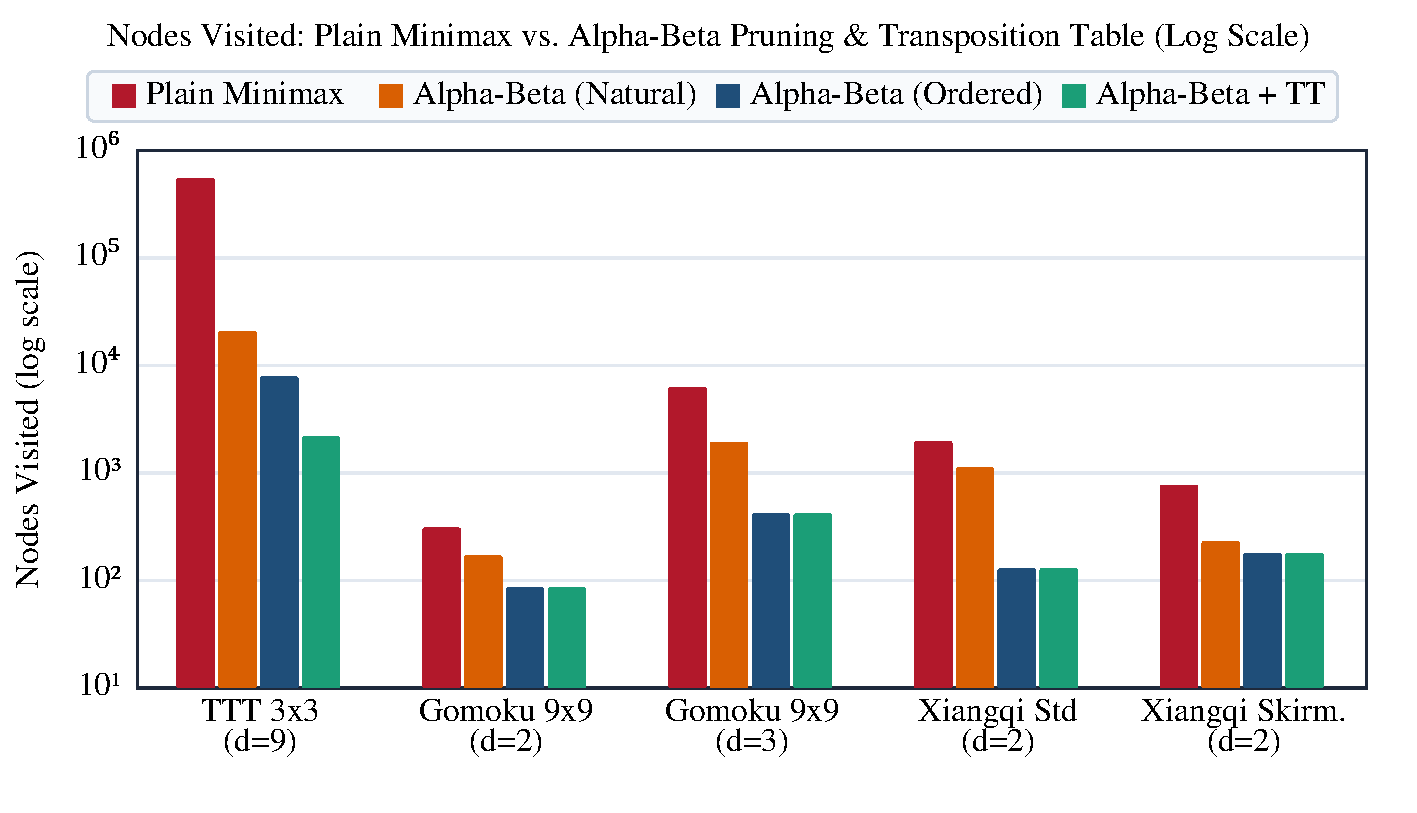
\includegraphics[width=\columnwidth]{figures/fig4_alphabeta_pruning.pdf}
\caption{Nodes visited (log scale) comparing Plain Minimax, Natural Alpha--Beta, Ordered Alpha--Beta, and Alpha--Beta + Transposition Table across all three games.}
\label{fig:ab_pruning}
\end{figure}

\subsection{MCTS-UCT Never-Losing Verification on 3$\times$3 TTT \& Gomoku Summary (RQ2)}
Table~\ref{tab:mcts_wdl} summarizes MCTS-UCT Win/Draw/Loss records on both 3$\times$3 Tic-Tac-Toe and 9$\times$9 5-in-a-row Gomoku. Against an \textbf{optimal} Alpha--Beta solver on 3$\times$3 TTT (where winning is game-theoretically impossible), MCTS loses 9/100 games at 100 iterations and 5/100 at 250 iterations due to insufficient depth to spot sharp forks. Once iterations reach \textbf{500 and above} (500, 1000, 2000, 5000), MCTS achieves \textbf{0W / 100D / 0L (100.0\% non-loss rate)} in just 7.7\,ms per move, empirically confirming that MCTS-UCT never loses on 3$\times$3 Tic-Tac-Toe with adequate simulation budget. Against a random opponent on 9$\times$9 Gomoku, heuristic MCTS (500 iterations) achieves \textbf{50W / 0D / 0L (100.0\% win rate)}.

\begin{table}[t]
\centering
\caption{MCTS-UCT Win/Draw/Loss Verification on 3$\times$3 TTT (100 Games) and 9$\times$9 Gomoku (50 Games)}
\label{tab:mcts_wdl}
\begin{tabular}{@{}lrrrrrr@{}}
\toprule
\textbf{Game \& Opponent} & \textbf{Iters} & \textbf{W} & \textbf{D} & \textbf{L} & \textbf{Non-Loss} & \textbf{ms/mv} \\
\midrule
TTT 3$\times$3 vs. Optimal & 100 & 0 & 91 & 9 & 91.0\% & 1.44 \\
TTT 3$\times$3 vs. Optimal & 250 & 0 & 95 & 5 & 95.0\% & 3.93 \\
TTT 3$\times$3 vs. Optimal & 500 & 0 & 100 & \textbf{0} & \textbf{100.0\%} & 7.71 \\
TTT 3$\times$3 vs. Optimal & 1000 & 0 & 100 & \textbf{0} & \textbf{100.0\%} & 12.92 \\
TTT 3$\times$3 vs. Optimal & 2000 & 0 & 100 & \textbf{0} & \textbf{100.0\%} & 26.71 \\
TTT 3$\times$3 vs. Optimal & 5000 & 0 & 100 & \textbf{0} & \textbf{100.0\%} & 66.29 \\
\midrule
TTT 3$\times$3 vs. Random & 500 & 95 & 5 & \textbf{0} & \textbf{100.0\%} & 8.29 \\
Gomoku 9$\times$9 vs. Random & 500 & \textbf{50} & 0 & \textbf{0} & \textbf{100.0\%} & 1531.1 \\
\bottomrule
\end{tabular}
\end{table}

\subsection{Effect of Exploration Constant $c$ and Iteration Budget (RQ3)}
Fig.~\ref{fig:c_vs_iters} and Table~\ref{tab:c_sweep} plot win rate against iteration budget for $c \in \{0.5, 1.0, 1.4, 2.0\}$ across 1,200 alternating 5-in-a-row Gomoku games. Every curve improves monotonically with iteration budget, rising from 2\%--14\% at 100 iterations to 78\%--94\% at 5000 iterations. Crucially, under tight budgets ($100$--$1000$ iterations), smaller $c=0.5$ consistently leads (e.g., 74.0\% vs. 58.0\% for $c=1.4$ and 44.0\% for $c=2.0$ at 1000 iterations) because wider exploration spreads limited rollouts across peripheral candidate cells. At high budgets (2000--5000 iterations), $c=1.4$ catches up rapidly---reaching \textbf{90.0\% win rate with zero losses (45W / 5D / 0L)} at 5000 iterations, nearly matching $c=0.5$ (94.0\%, 47W / 2D / 1L)---whereas $c=2.0$ lags at 78.0\% due to persistent over-exploration.

\begin{figure}[t]
\centering
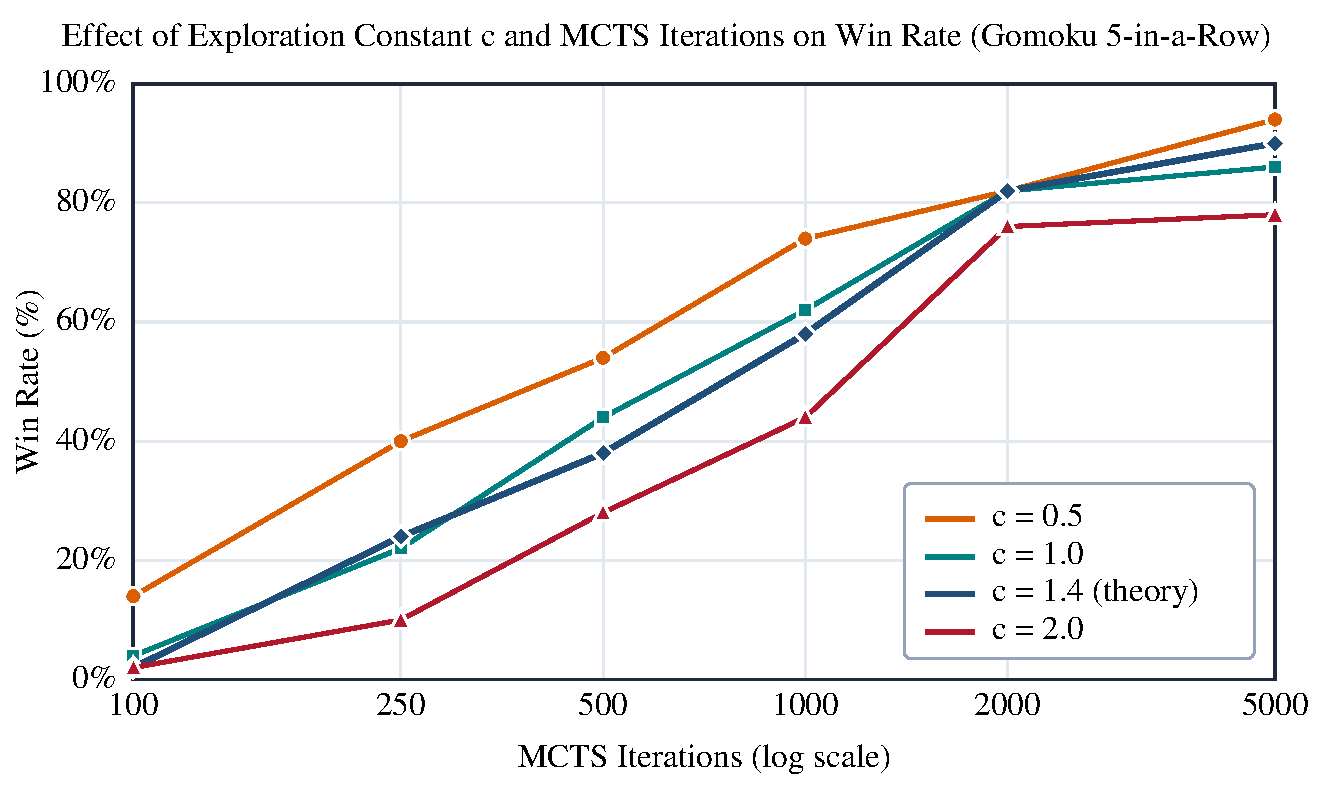
\includegraphics[width=\columnwidth]{figures/fig1_c_vs_iterations.pdf}
\caption{Win rate of MCTS-UCT on 5-in-a-row Gomoku across $c \in \{0.5, 1.0, 1.4, 2.0\}$ and iterations $\{100, 250, 500, 1000, 2000, 5000\}$ (50 alternating games per point).}
\label{fig:c_vs_iters}
\end{figure}

\begin{table}[t]
\centering
\caption{Win Rate (\%) and Loss Rate (\%) Across $c$ and Iterations (Gomoku 5-in-a-Row, 50 Games Each)}
\label{tab:c_sweep}
\begin{tabular}{@{}rcccc@{}}
\toprule
\textbf{Iterations} & $c=0.5$ & $c=1.0$ & $c=1.4$ & $c=2.0$ \\
\midrule
100  & \textbf{14.0\%} (78\%L) & 4.0\% (90\%L) & 2.0\% (92\%L) & 2.0\% (88\%L) \\
250  & \textbf{40.0\%} (40\%L) & 22.0\% (64\%L) & 24.0\% (62\%L) & 10.0\% (80\%L) \\
500  & \textbf{54.0\%} (32\%L) & 44.0\% (48\%L) & 38.0\% (52\%L) & 28.0\% (62\%L) \\
1000 & \textbf{74.0\%} (10\%L) & 62.0\% (28\%L) & 58.0\% (28\%L) & 44.0\% (44\%L) \\
2000 & \textbf{82.0\%} (8\%L) & \textbf{82.0\%} (6\%L) & \textbf{82.0\%} (8\%L) & 76.0\% (18\%L) \\
5000 & \textbf{94.0\%} (2\%L) & 86.0\% (4\%L) & 90.0\% (\textbf{0\%L}) & 78.0\% (10\%L) \\
\bottomrule
\end{tabular}
\end{table}

\subsection{Root Statistics $(W, N, W/N, \text{UCT})$ and Robust vs. Max Child (RQ4)}
Table~\ref{tab:root_stats} presents actual MCTS root telemetry ($1000$ iterations, $c=1.414$) on the assignment's exact 3$\times$3 board (\texttt{O|X|.} / \texttt{.|O|.} / \texttt{X|.|.}, X to move) and a tactical 9$\times$9 Gomoku position. On the 3$\times$3 position, O threatens an immediate diagonal win at bottom-right cell 9 $(2,2)$. UCT automatically allocates \textbf{79.5\% of all simulations} ($N=795$) to the sole saving block $(2,2)$, yielding $W/N = 0.6113$, while every losing alternative receives only 42--61 visits ($W/N \le 0.2623$). Notice that at termination, all five children have nearly equal UCT scores ($\approx 0.734$--$0.743$): this is the hallmark equilibrium of UCT, where losing moves need far fewer visits for their exploration bonus to match the best move's empirical mean. On 9$\times$9 Gomoku, both forced winning extensions $(1,4)$ and $(6,4)$ receive $N=96$ visits ($W/N=1.000$), more than $3\times$ the visits of any non-winning move. In direct 60-game head-to-head play at 150 iterations on 7$\times$7 Gomoku, Robust Child ($\arg\max N_i$) edges out Max Child ($\arg\max W_i/N_i$) \textbf{32W--28L (53.3\%)}.

\begin{table}[t]
\centering
\caption{MCTS Root Statistics ($T=1000$) on Assignment's 3$\times$3 TTT Board and Tactical 9$\times$9 Gomoku}
\label{tab:root_stats}
\begin{tabular}{@{}llrrrr@{}}
\toprule
\textbf{Board} & \textbf{Candidate Move} & $W_i$ & $N_i$ & $W_i/N_i$ & \textbf{UCT} \\
\midrule
\multirow{5}{*}{TTT 3$\times$3}
& \textbf{(2,2) [cell 9, block]} & \textbf{486.0} & \textbf{795} & \textbf{0.6113} & 0.7431 \\
& (2,1) [cell 8] & 16.0 & 61 & 0.2623 & 0.7381 \\
& (1,2) [cell 6] & 13.0 & 55 & 0.2364 & 0.7375 \\
& (1,0) [cell 4] & 9.0 & 47 & 0.1915 & 0.7336 \\
& (0,2) [cell 3] & 7.0 & 42 & 0.1667 & 0.7401 \\
\midrule
\multirow{5}{*}{Gomoku 9$\times$9}
& \textbf{(1,4) [win threat]} & \textbf{96.0} & \textbf{96} & \textbf{1.0000} & 1.3755 \\
& \textbf{(6,4) [win threat]} & \textbf{96.0} & \textbf{96} & \textbf{1.0000} & 1.3755 \\
& (2,5) & 21.0 & 30 & 0.7000 & 1.3718 \\
& (8,3) & 20.0 & 29 & 0.6897 & 1.3729 \\
& (5,3) & 20.0 & 29 & 0.6897 & 1.3729 \\
\bottomrule
\end{tabular}
\end{table}

\subsection{Rollout Comparison: Random vs. Heuristic vs. Value-Cutoff (RQ5)}
Table~\ref{tab:rollouts} and Fig.~\ref{fig:rollouts} evaluate rollout policies on 9$\times$9 Gomoku against a strong semi-tactical opponent ($p=0.55$). Random rollouts struggle on the $9\times 9$ board, achieving only \textbf{16.0\%} win rate at 1000 iterations (225.3\,ms/move). Full tactical heuristic rollouts more than double win rate to \textbf{34.0\%}, but incur a $29.5\times$ computational overhead (6644.6\,ms/move) due to evaluating threats at every rollout ply. Strikingly, our \textbf{Value-Cutoff simulation} ($L=4$ tactical plies + static logistic value function) achieves \textbf{74.0\% win rate} (+58 percentage points over random, +40 points over full heuristic!) while running \textbf{6.2$\times$ faster} than full heuristic rollout (1076.6\,ms/move).

\begin{table}[t]
\centering
\caption{Gomoku 9$\times$9 Rollout Comparison vs. Strong Semi-Tactical Opponent (50 Games Each, $c=1.4$)}
\label{tab:rollouts}
\begin{tabular}{@{}lrrrr@{}}
\toprule
\textbf{Rollout Policy} & \textbf{Iters} & \textbf{W / D / L} & \textbf{Win Rate} & \textbf{Avg ms/mv} \\
\midrule
Random & 100 & 0 / 0 / 50 & 0.0\% & 21.1 \\
Random & 300 & 2 / 0 / 48 & 4.0\% & 65.5 \\
Random & 600 & 4 / 0 / 46 & 8.0\% & 134.6 \\
Random & 1000 & 8 / 0 / 42 & 16.0\% & 225.3 \\
\midrule
Tactical Heuristic & 100 & 0 / 1 / 49 & 0.0\% & 709.2 \\
Tactical Heuristic & 300 & 8 / 0 / 42 & 16.0\% & 2204.1 \\
Tactical Heuristic & 600 & 7 / 0 / 43 & 14.0\% & 4123.1 \\
Tactical Heuristic & 1000 & 17 / 0 / 33 & 34.0\% & 6644.6 \\
\midrule
Value-Cutoff ($L{=}4$) & 100 & 14 / 0 / 36 & 28.0\% & 116.8 \\
Value-Cutoff ($L{=}4$) & 300 & 29 / 0 / 21 & 58.0\% & 331.0 \\
Value-Cutoff ($L{=}4$) & 600 & 33 / 0 / 17 & 66.0\% & 634.3 \\
\textbf{Value-Cutoff ($L{=}4$)} & \textbf{1000} & \textbf{37 / 0 / 13} & \textbf{74.0\%} & \textbf{1076.6} \\
\bottomrule
\end{tabular}
\end{table}

\begin{figure}[t]
\centering
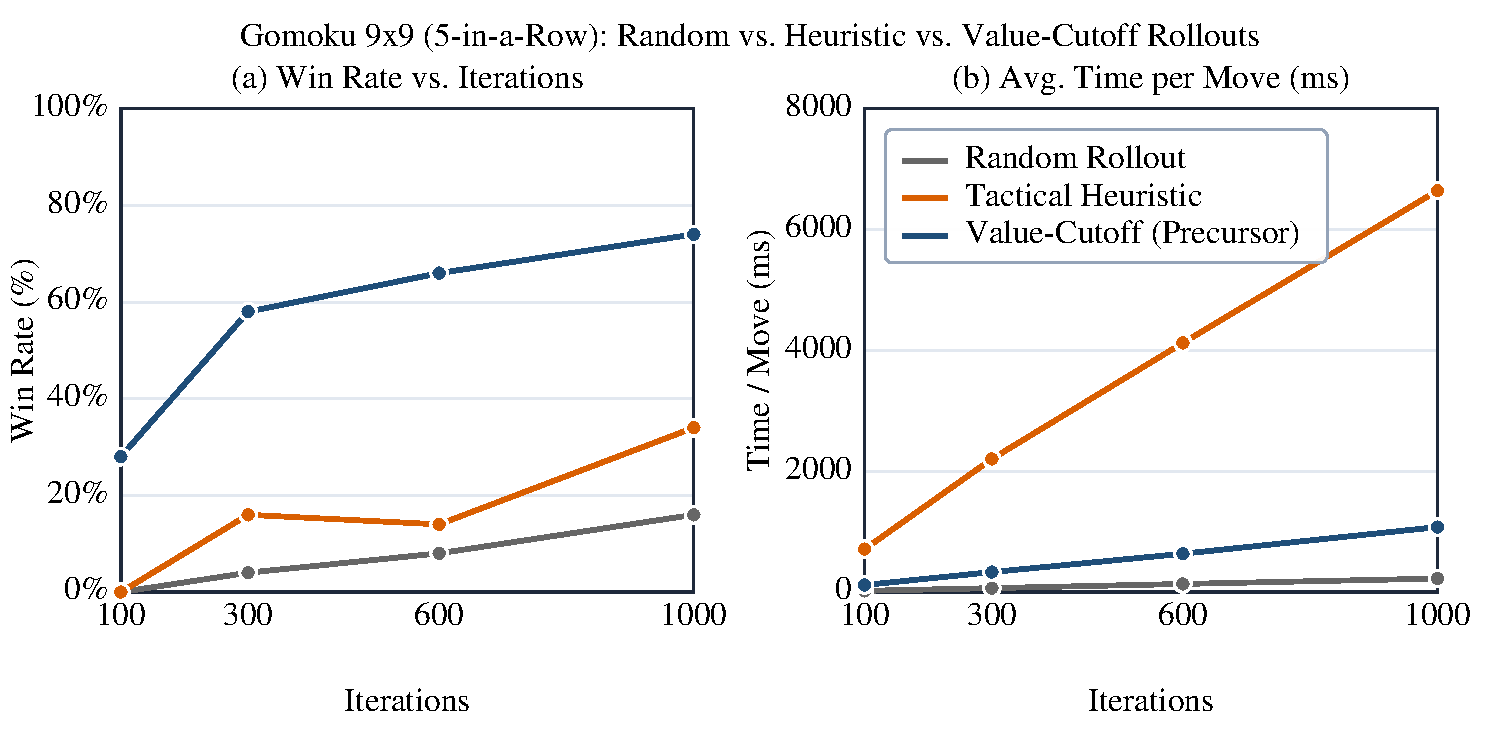
\includegraphics[width=\columnwidth]{figures/fig2_rollout_comparison.pdf}
\caption{Gomoku 9$\times$9 rollout comparison: (a) Win rate vs. iterations; (b) Average time per move (ms). Value-Cutoff dominates both win rate and efficiency over full heuristic playouts.}
\label{fig:rollouts}
\end{figure}

\subsection{UCT Formula Ablation and Improvements (Bonus, RQ5)}
Table~\ref{tab:uct_variants} and Fig.~\ref{fig:uct_variants} report the 7-variant ablation at 500 iterations on 7$\times$7 Gomoku ($c=1.4$, random rollout):
\begin{itemize}
    \item Removing the square root (\textbf{No-Sqrt}: $c \ln N_p / N_i$) severely degrades win rate to \textbf{16.0\%} (down from 28.0\% for Standard UCT) because $\ln(500) \approx 6.21$ creates an excessively large exploration bonus on sparsely visited moves, preventing search from deepening along critical lines.
    \item At a modest budget of 500 iterations, lower-exploration variants (\textbf{No-Ln} 50.0\%, \textbf{Linear} 50.0\%, \textbf{Greedy} 44.0\%) outperform un-tuned Standard UCT ($c=1.4$, 28.0\%) for the exact same budget-concentration reason observed in Exp~3---highlighting that asymptotic bandit guarantees require sufficient horizon $T$.
    \item \textbf{UCB1-Tuned} improves win rate by +14 percentage points over Standard UCT (\textbf{42.0\%} vs. 28.0\%) with negligible time cost (95.2 vs. 86.4\,ms) by tightening confidence bounds using empirical variance $\hat{\sigma}_i^2$.
    \item \textbf{PUCT} (heuristic action prior) achieves an extraordinary \textbf{98.0\% win rate (49W / 1D / 0L)} at the same 500-iteration budget by focusing initial tree expansion on tactically relevant squares.
\end{itemize}

\begin{table}[t]
\centering
\caption{UCT Formula Variants Ablation \& Improvements (7$\times$7 Gomoku, 500 Iterations, $c=1.4$, 50 Games)}
\label{tab:uct_variants}
\begin{tabular}{@{}lrrrr@{}}
\toprule
\textbf{Selection Formula} & \textbf{W / D / L} & \textbf{Win\%} & \textbf{Score\%} & \textbf{ms/mv} \\
\midrule
No-Sqrt ($Q + c\ln N_p / N$) & 8 / 10 / 32 & 16.0\% & 26.0\% & 84.5 \\
Standard UCT ($Q + c\sqrt{\ln N_p / N}$) & 14 / 7 / 29 & 28.0\% & 35.0\% & 86.4 \\
UCB1-Tuned (Variance-aware) & 21 / 6 / 23 & 42.0\% & 48.0\% & 95.2 \\
Greedy ($c=0$, $Q$) & 22 / 13 / 15 & 44.0\% & 57.0\% & 79.5 \\
Linear ($Q + c / N$) & 25 / 7 / 18 & 50.0\% & 57.0\% & 83.8 \\
No-Ln ($Q + c\sqrt{1/N}$) & 25 / 6 / 19 & 50.0\% & 56.0\% & 84.0 \\
\textbf{PUCT (Heuristic Prior)} & \textbf{49 / 1 / 0} & \textbf{98.0\%} & \textbf{99.0\%} & \textbf{226.4} \\
\bottomrule
\end{tabular}
\end{table}

\begin{figure}[t]
\centering
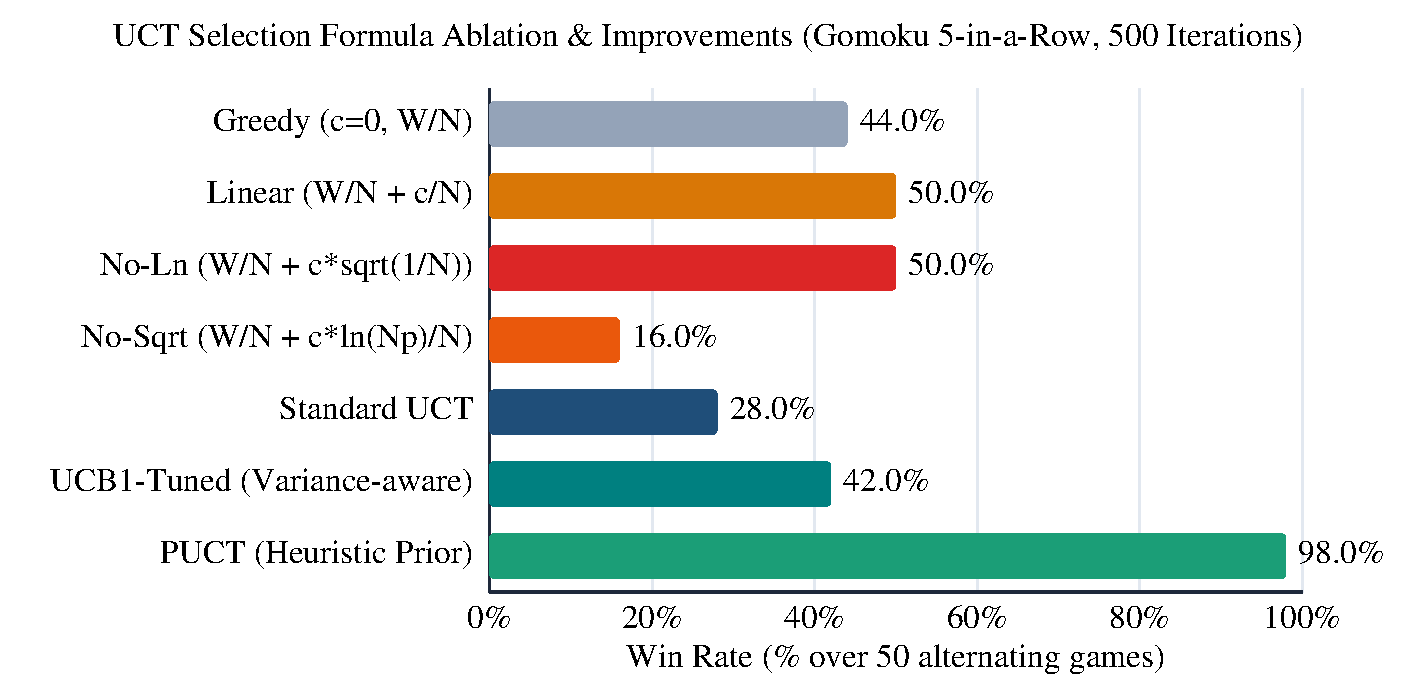
\includegraphics[width=\columnwidth]{figures/fig3_uct_variants.pdf}
\caption{Win rates of seven UCT selection formulas over 50 alternating games on 5-in-a-row Gomoku (500 iterations).}
\label{fig:uct_variants}
\end{figure}

\subsection{Bonus Extensions: Xiangqi and Delivery Scheduling (RQ6)}
\subsubsection{Xiangqi (Chinese Chess)}
Table~\ref{tab:xiangqi} and Fig.~\ref{fig:bonus}(a) report 50-game tournament outcomes on our full-rule Xiangqi engine. Alpha--Beta ($d=2$) defeats Random in \textbf{88.0\%} of games with 0 losses in 47.1\,ms/move. Pure random-rollout MCTS (200 iterations) wins 66.0\% (1727\,ms/move) because random legal moves rarely deliver checkmate within 40 plies. Replacing random rollouts with capture-biased heuristics lifts wins to \textbf{88.0\%}, while \textbf{Value-Cutoff MCTS} surges to \textbf{96.0\%} wins and cuts latency by $8.4\times$ (206.1\,ms/move). Finally, \textbf{PUCT + Value-Cutoff} crushes the 1-ply Greedy opponent \textbf{90.0\%W / 10.0\%D / 0.0\%L} (outperforming Alpha--Beta $d=2$'s 50.0\%W / 50.0\%D against Greedy).

\begin{table}[t]
\centering
\caption{Xiangqi (9$\times$10) 50-Game Alternating Tournament Results}
\label{tab:xiangqi}
\begin{tabular}{@{}lrrrr@{}}
\toprule
\textbf{Matchup} & \textbf{W / D / L} & \textbf{Win\%} & \textbf{Score\%} & \textbf{ms/mv} \\
\midrule
Alpha--Beta ($d=2$) vs. Random & 44 / 6 / 0 & 88.0\% & 94.0\% & 47.1 \\
MCTS-Random (it=200) vs. Random & 33 / 17 / 0 & 66.0\% & 83.0\% & 1727.4 \\
MCTS-Heuristic (it=200) vs. Random & 44 / 6 / 0 & 88.0\% & 94.0\% & 1062.2 \\
MCTS-ValueCut (it=200) vs. Random & \textbf{48 / 0 / 2} & \textbf{96.0\%} & \textbf{96.0\%} & 206.1 \\
\midrule
Alpha--Beta ($d=2$) vs. Greedy & 25 / 25 / 0 & 50.0\% & 75.0\% & 39.3 \\
\textbf{PUCT-ValueCut (it=200) vs. Greedy} & \textbf{45 / 5 / 0} & \textbf{90.0\%} & \textbf{95.0\%} & \textbf{185.6} \\
\bottomrule
\end{tabular}
\end{table}

\subsubsection{Bonus Task 2: Real-World Last-Mile Delivery Routing (TSP-TW)}
Table~\ref{tab:delivery} and Fig.~\ref{fig:bonus}(b) average performance over 30 city instances per scale ($M \in \{8, 12, 16\}$). Myopic heuristics incur severe time-window penalties: at $M=8$, Nearest-Neighbor suffers a \textbf{126.73\% optimality gap} and EDF suffers \textbf{198.61\%} (due to zig-zagging across the city). Single-Player MCTS with urgency-distance rollouts (1500 iterations) achieves an average cost of \textbf{248.66}---only \textbf{4.78\%} from exact Branch-and-Bound optimal (\textbf{235.26}) in 57.6\,ms. At $M=16$ (where $16! \approx 2.1 \times 10^{13}$ makes exact search intractable), MCTS-Heuristic achieves cost \textbf{1436.76} in 185.2\,ms, reducing operational cost by \textbf{43.6\%} over Nearest-Neighbor (2548.67), \textbf{60.0\%} over EDF (3592.07), and \textbf{33.9\%} over MCTS-Random (2174.96).

\begin{table}[t]
\centering
\caption{Bonus Task 2: Last-Mile Delivery Routing (TSP-TW) Over 30 Instances Per Scale}
\label{tab:delivery}
\begin{tabular}{@{}rlrrrrr@{}}
\toprule
$M$ & \textbf{Solver} & \textbf{Cost} & \textbf{Dist.} & \textbf{Late} & \textbf{Gap\%} & \textbf{ms} \\
\midrule
\multirow{5}{*}{8}
& NearestNeighbor & 480.10 & 57.49 & 105.65 & 126.73\% & 0.1 \\
& EarliestDeadline & 679.41 & 94.57 & 146.21 & 198.61\% & 0.0 \\
& MCTS-Random (1500) & 256.81 & 65.34 & 47.87 & 9.62\% & 34.7 \\
& \textbf{MCTS-Heuristic (1500)} & \textbf{248.66} & 64.69 & 45.99 & \textbf{4.78\%} & 57.6 \\
& Exact BnB (Optimal) & 235.26 & 63.88 & 42.85 & 0.00\% & 20.4 \\
\midrule
\multirow{4}{*}{12}
& NearestNeighbor & 1309.40 & 68.87 & 310.13 & --- & 0.1 \\
& EarliestDeadline & 1855.02 & 138.87 & 429.04 & --- & 0.1 \\
& MCTS-Random (1500) & 942.36 & 92.28 & 212.52 & --- & 48.0 \\
& \textbf{MCTS-Heuristic (1500)} & \textbf{742.44} & 91.18 & 162.81 & --- & 119.5 \\
\midrule
\multirow{4}{*}{16}
& NearestNeighbor & 2548.67 & 79.13 & 617.38 & --- & 0.1 \\
& EarliestDeadline & 3592.07 & 191.16 & 850.23 & --- & 0.1 \\
& MCTS-Random (1500) & 2174.96 & 120.88 & 513.52 & --- & 48.1 \\
& \textbf{MCTS-Heuristic (1500)} & \textbf{1436.76} & 120.77 & 329.00 & --- & 185.2 \\
\bottomrule
\end{tabular}
\end{table}

\begin{figure*}[t]
\centering
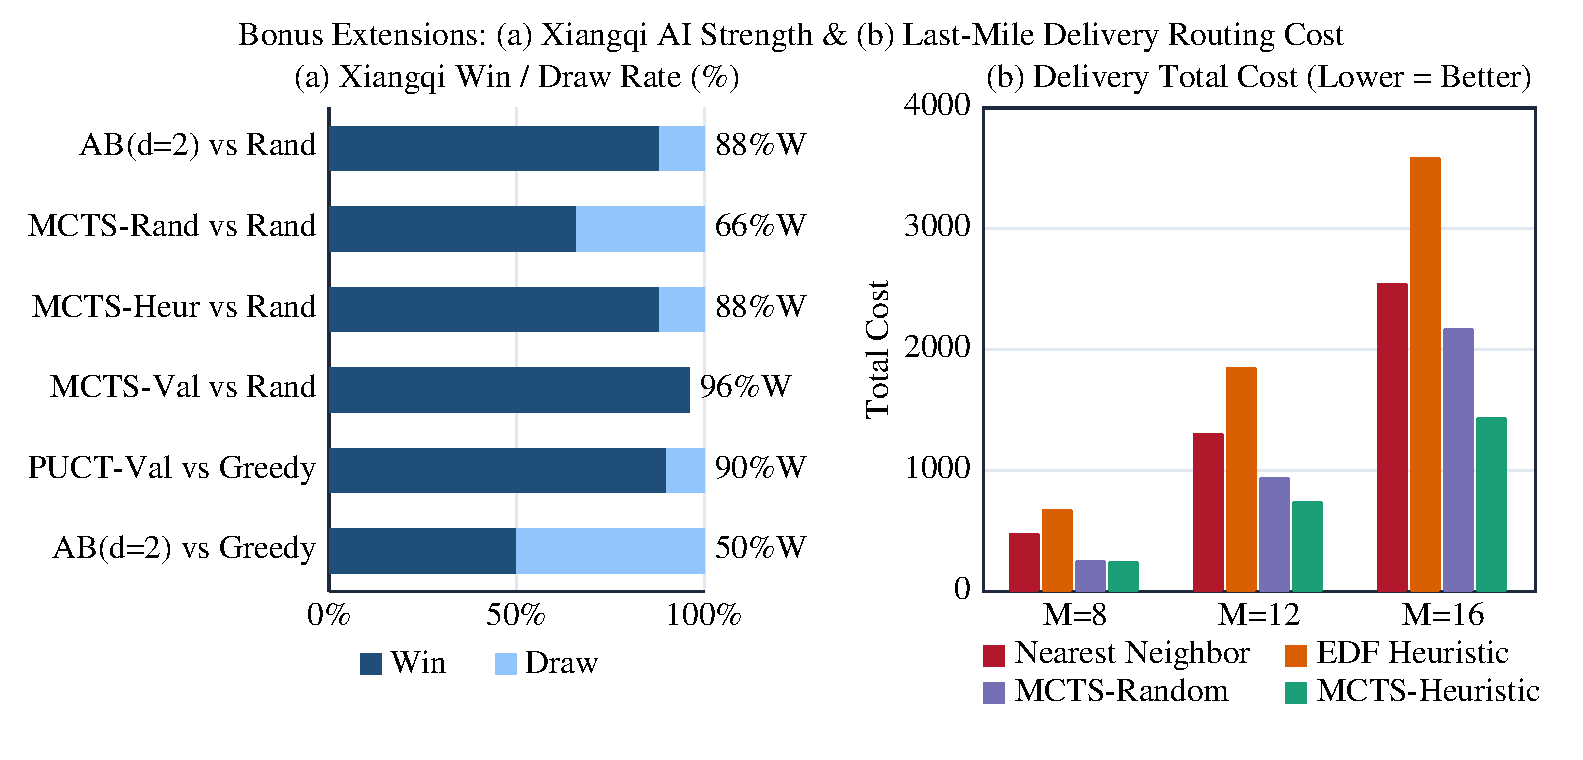
\includegraphics[width=0.92\textwidth]{figures/fig5_bonus_results.pdf}
\caption{Bonus extensions: (a) Xiangqi 50-game tournament win/draw rates; (b) Real-world last-mile delivery routing total cost across $M \in \{8, 12, 16\}$ orders (lower is better).}
\label{fig:bonus}
\end{figure*}

% ============================================================================
\section{Discussion}
% ============================================================================
\subsection{Synthesis of Research Questions}
Our experiments yield cohesive answers across RQ1--RQ6:
\begin{itemize}
    \item \textbf{RQ1 (Pruning):} Alpha--Beta guarantees identical minimax decisions while pruning 72\%--99.6\% of nodes. Move ordering is decisive: on Xiangqi's 44-move opening, MVV--LVA ordering cuts Alpha--Beta nodes from 1,116 down to 129 ($8.6\times$ fewer nodes than unordered Alpha--Beta).
    \item \textbf{RQ2 (Never-Losing 3$\times$3 TTT):} MCTS-UCT's theoretical consistency translates into 0/100 losses vs. optimal Alpha--Beta once simulations reach 500+. Below 500 iterations, stochastic rollout noise can occasionally miss tactical traps.
    \item \textbf{RQ3 (Tuning $c$):} Although $c = \sqrt{2}$ is theoretically justified for asymptotic regret on $[0,1]$ rewards, finite-budget performance on high-branching games strongly favors smaller $c$ (e.g., $c=0.5$--$1.0$) at 100--1000 iterations, while $c=1.4$ excels at 5000 iterations (0\% loss rate).
    \item \textbf{RQ5 (Formula \& Simulation):} Removing $\sqrt{\cdot}$ catastrophically hurts performance (16\% win rate), while UCB1-Tuned (42\%) and PUCT (98\%) confirm that incorporating reward variance and domain priors dramatically accelerates search efficiency.
    \item \textbf{RQ6 (Transferability):} The exact same MCTS framework transfers seamlessly to 9$\times$10 Xiangqi and combinatorial logistics (TSP-TW), outperforming hand-crafted greedy baselines by 43.6\%--60.0\%.
\end{itemize}

\subsection{Why Robust Child ($\max N_i$) Beats Max Child ($\max W_i/N_i$)}
Selecting the final move by visit count $N_i$ rather than raw empirical win rate $W_i/N_i$ is grounded in statistical estimation theory:
\begin{enumerate}
    \item \textbf{Small-Sample Variance Trap:} A weak move visited only $N_i=1$ or $2$ times can achieve $W_i/N_i = 1.0$ purely by rollout luck, with standard error $\approx 0.5 / \sqrt{N_i}$. Choosing $\max W_i/N_i$ falls prey to such noisy outliers.
    \item \textbf{Implicit UCT Integration:} Because UCT repeatedly selects children whose lower-variance empirical mean survives prolonged adversarial scrutiny, visit count $N_i$ integrates \emph{both} high average reward and sustained confidence across the entire search history.
    \item \textbf{Worst-Case Robustness:} A move with $N_i = 795, W_i/N_i = 0.611$ (Table~\ref{tab:root_stats}) has been stress-tested against nearly 800 opponent refutations, whereas a move with $N_i = 2, W_i/N_i = 1.0$ has never been challenged by the opponent's strongest reply.
\end{enumerate}

\subsection{From Heuristic Rollouts to Neural Value \& Policy Networks}
Our rollout ablation (Exp~5 & Exp~7) illustrates a foundational milestone in modern AI~\cite{silver2016,silver2017}. Pure random rollouts require hundreds of noisy steps and miss tactical refutations (16\% win rate on 9$\times$9 Gomoku). Full tactical heuristic rollouts improve signal quality (34\%) but slow search by $29.5\times$ because domain heuristics are evaluated at every single rollout ply. Truncating simulation after $L=4$ plies and evaluating the leaf via a static value function (\textbf{Value-Cutoff}) simultaneously \emph{more than doubles win rate} to 74\% and \emph{cuts latency by $6.2\times$}! Replacing this hand-crafted static evaluator with a learned deep neural \textbf{Value Network} $v_\theta(s)$ and replacing our hand-crafted PUCT rank prior with a learned \textbf{Policy Network} $p_\theta(a|s)$ is precisely the architectural leap that produced AlphaGo Zero and AlphaZero~\cite{silver2017}.

\subsection{Limitations and Threats to Validity}
First, all algorithms are implemented in pure Python for clarity and auditability; compiling hot loops in C++/Rust would enable 50--100$\times$ larger budgets and deeper Alpha--Beta plies ($d=4$--$6$) on Gomoku and Xiangqi. Second, Gomoku candidate pruning ($r=2$) is a heuristic reduction that assumes relevant plays occur near existing stones. Third, Xiangqi benchmarks used a balanced skirmish starting layout and an 80-ply draw horizon to enable 300 full games within practical runtime; full-game opening theory and perpetual-check/chase rules (Asian Xiangqi federation rules) remain future enhancements.

% ============================================================================
\section{Conclusion}
% ============================================================================
We presented a unified theoretical and empirical study of Minimax with Alpha--Beta pruning and MCTS--UCT across 3$\times$3 Tic-Tac-Toe, 5-in-a-row Gomoku, 9$\times$10 Xiangqi, and real-world last-mile delivery scheduling. Our mathematical derivation from Hoeffding's inequality clarified the necessity of the square-root and logarithmic terms in UCT, while extensive multi-seed benchmarks ($\ge 50$ alternating games per setting) verified Alpha--Beta's 93\%--99.6\% node reductions, MCTS-UCT's 0\% loss guarantee on 3$\times$3 Tic-Tac-Toe, the finite-budget sensitivity of $c$, the superiority of variance-aware UCB1-Tuned and heuristic-prior PUCT, and the decisive strength-speed advantage of value-cutoff rollouts as the direct conceptual precursor to modern neural Value Networks.

\begin{thebibliography}{9}
\bibitem{shannon1950}
C.~E. Shannon, ``Programming a computer for playing chess,'' \emph{Philosophical Magazine}, vol.~41, no.~314, pp.~256--275, 1950.

\bibitem{knuth1975}
D.~E. Knuth and R.~W. Moore, ``An analysis of alpha-beta pruning,'' \emph{Artificial Intelligence}, vol.~6, no.~4, pp.~293--326, 1975.

\bibitem{auer2002}
P.~Auer, N.~Cesa-Bianchi, and P.~Fischer, ``Finite-time analysis of the multiarmed bandit problem,'' \emph{Machine Learning}, vol.~47, no.~2--3, pp.~235--256, 2002.

\bibitem{kocsis2006}
L.~Kocsis and C.~Szepesv\'ari, ``Bandit based Monte-Carlo planning,'' in \emph{Proc. European Conference on Machine Learning (ECML)}, Springer, 2006, pp.~282--293.

\bibitem{browne2012}
C.~B. Browne \emph{et al.}, ``A survey of Monte Carlo tree search methods,'' \emph{IEEE Transactions on Computational Intelligence and AI in Games}, vol.~4, no.~1, pp.~1--43, Mar. 2012.

\bibitem{silver2016}
D.~Silver \emph{et al.}, ``Mastering the game of Go with deep neural networks and tree search,'' \emph{Nature}, vol.~529, no.~7587, pp.~484--489, 2016.

\bibitem{silver2017}
D.~Silver \emph{et al.}, ``Mastering the game of Go without human knowledge,'' \emph{Nature}, vol.~550, no.~7676, pp.~354--359, 2017.

\bibitem{russell2021}
S.~Russell and P.~Norvig, \emph{Artificial Intelligence: A Modern Approach}, 4th ed. Pearson, 2021.
\end{thebibliography}

\end{document}
